\documentclass[../main.tex]{subfiles}

\begin{document}

\section{Kompaktní prostory}

\begin{definition}[Kompaktní metrický prostor]
	Metrický prostor $(X,d)$ je kompaktní, pokud každá posloupnost v něm obsahuje konvergentní podposloupnost.
\end{definition}

\subsection{Vlastnosti kompaktních prostorů}

\begin{lemma}[Podprostor kompaktního prostoru]
	Podprostor kompaktního prostoru je kompaktní právě když je uzavřený.
\end{lemma}

\begin{proof}
	\begin{enumerate}
	    \item[$\Leftarrow \phantom{\lnot} $] Buď $Y$ uzavřený podprostor kompaktního $X$ a buď $(y_n)_n$ posloupnost v $Y$. Jako posloupnost v X má 
	    konvergentní podposloupnost s limitou a z uzavřenosti je konvergentní podposloupností a tato limita je v $Y$.
	    \item[$\lnot \Leftarrow \lnot $] Nechť $Y$ není uzavřený. Potom existuje posloupnost $(y_n)_n$ v $Y$ konvergentní v $X$ taková, že $y = \lim_n y_n \notin Y$. Potom $(y_n)_n$
	    nemůže mít podposloupnost konvergentní v $Y$ protože každá její podposloupnost konverguje k $y$.
	\end{enumerate}
\end{proof}

\begin{lemma}[Uzavřenost kompaktního podprostoru] \label{ch:komp=>uz}
	Buď $(X,d)$ libovolný metrický prostor a
	buď podprostor $Y \subseteq X$ kompaktní. Potom $Y$ je uzavřený v $(X,d)$.
\end{lemma}

\begin{proof}
	Nechť $(y_n)_n$ posloupnost v $Y$ konverguje v $X$ k limitě $y$. Potom každá podposloupnost $(y_n)_n$ konverguje k 
	$y$ a tedy je $y \in Y$.
\end{proof}

\begin{theorem}[Součin kompaktních prostorů]
	Součin konečně mnoha kompaktních prostorů je kompaktní.
\end{theorem}

\begin{proof}
	Stačí dokázat pro součin dvou prostorů (součin prostorů je komutativní).
	Buďte $(X,d_1), (X, d_2)$ kompaktní a buď $((x_n,y_n))_n$ posloupnost v $X \times Y$. 
	Zvolme konvergentní podposloupnost $(x_{k_n})_n$ posloupnosti $(x_n)_n$ a konvergentní podposloupnost $(y_{k_{l_n}})_n$ posloupnosti $(y_{k_n})_n$.
	Potom je 
	\[((x_{k_{l_n}},y_{k_{l_n}}))_n\]
	konvergentní podposloupnost posloupnosti $((x_n,y_n))_n$.
\end{proof}

\subsection{Omezené metrické prostory}

\begin{definition}[Omezený metrický prostor]
	Metrický prostor $(X,d)$ je omezený, jestliže pro nějaké $K$ platí
	\[\forall x,y \in X : d(x,y) < K.\]
\end{definition}

\begin{lemma}[Omezenost kompaktního prostoru]\label{ch:komp=>om}
	Každý kompaktní prostor je omezený.
\end{lemma}

\begin{proof}
	Zvolme $x_1$ libovolně a $x_n$ tak, aby $d(x_1,x_n) > n$. Posloupnost $(x_n)_n$ nemá konvergentní podposloupnost; kdyby $x$
	byla limita takové podposloupnosti, bylo by pro dost velké $n$ nekonečně mnoho členů této podposloupnosti blíže k $x_1$ než $d(x_1,x_n)+1$, což je spor.
\end{proof}

\subsection{Euklidovské metrické prostory}
\begin{remark}
	Kompaktní interval v $\mathbb{E}_n$: součin intervalů $\left<a_i,b_i\right>$.
\end{remark}

\begin{theorem}[Kompaktnost podprostoru $\mathbb{E}$]
	Podprostor euklidovského prostoru $\mathbb{E}_n$ je kompaktní právě když je uzavřený a omezený.
\end{theorem}

\begin{proof}
	\begin{enumerate}
		\item[$\Rightarrow$:] Že je uzavřený a omezený už víme (\ref{ch:komp=>uz}, \ref{ch:komp=>om}).
		\item[$\Leftarrow$:] Buď nyní $Y \subseteq \mathbb{E}_n$ omezený a uzavřený. Jelikož je omezený, tak pro dostatečně velký kompaktní interval platí
	    \[Y \subseteq J^n \subseteq \mathbb{E}_n.\]
	    $J^n$ je kompaktní jako součin intervalů $\left<a_i,b_i\right>$, a jelikož je $Y$ uzavřený v $\mathbb{E}_n$ je též uzavřený
	    v $J^n$ a tedy kompaktní.
	\end{enumerate}
\end{proof}

\subsection{Spojitá zobrazení}

\begin{lemma}[Obraz spojitého zobrazení na kompaktním prostoru]
	Buď $f: (X,d) \to (Y, d')$ spojité zobrazení a buď $A \subseteq X$ kompaktní. Potom je $f[A]$ kompaktní.
\end{lemma}

\begin{proof}
	Buď $(y_n)_n$ posloupnost v $f[A]$. Zvolme $x_n \in A$ tak, aby $y_n = f(x_n)$. Buď $(x_{k_n})_n$ konvergentní podposloupnost
	Potom je $(y_{k_n})_n = (f(x_{k_n}))_n$ konvergentní podposloupnost $(x_n)_n$.
\end{proof}

\begin{lemma}[Extrémy spojité funkce na kompaktním prostoru]
	Buď $(X,d)$ kompaktní. Potom každá spojitá funkce $f:(X,d)\to \mathbb{R}$ nabývá maxima i minima (t.j. nejsou nekonečné).
\end{lemma}

\begin{proof}
	Buď $Y = f[X] \subseteq \mathbb{R}$ kompaktní. Je to tedy omezená množina a musí mít supremum $M\in \mathbb{R}$ a infimum $m\in \mathbb{R}$. Zřejmě máme 
	$d(m,Y) = d(M,Y) = 0$ a jelikož $Y$ je uzavřená, $m,M \in Y$. Víme, že spojitá $f$ je charakterizována tím, že všechny vzory uzavřených množin
	jsou uzavřené. Nyní vidíme, že je-li definiční obor kompaktní, platí též, že obrazy uzavřených podmnožin jsou uzavřené. 
\end{proof}

% TODO: z čeho to plyne? To spíš z obrazu spojitého zobrazení, ne?
% Z toho plyne následujíci:

\begin{theorem}[Vzájemně jednoznačné spojité zobrazení]
	Je-li $(X,d)$ kompaktní a je-li $f: (X,d) \to (Y,d')$ vzájemně jednoznačné spojité zobrazení, pak je
	$f$ homeomorfismus.\footnote{
	Obecněji: Nechť $f:(X,d) \to (Y,d')$ je spojité a na. Mějme potom $g: (X,d) \to (Z, d'')$ spojité a
	$h: (Y,d') \to (Z,d'')$ takové, že $h \circ f = g$. Potom je $h$ spojité.}
\end{theorem}

\begin{proof}
	Buď $B$ uzavřená v $Z$. Potom je $A = g^{-1}[B]$ uzavřená $\implies$ kompaktnost v $X$ $\implies$ $f[A]$ je kompaktní $\implies$ uzavřená v $Y$. Jelikož  je $f$ zobrazení na, máme $f[f^{-1}[C]] = C\ \forall C$. Proto je 
	\[h^{-1}[B] = f[f^{-1}[h^{-1}[B]]] = f[(h \circ f)^{-1}[B]] = f[g^{-1}[B]] = f[A]\]
	uzavřená.
\end{proof}

\subsection{Cauchyovské posloupnosti}

\begin{definition}[Cauchyovská posloupnost]
	Posloupnost $(x_n)_n$ v $(X,d)$ je Cauchyovská, jestliže
	\[ \forall \varepsilon > 0\ \exists n_0: m,n \geq n_0 \implies d(x_m, x_n) < \varepsilon \]
\end{definition}

\begin{intuition}
	Vlastnost popisuje posloupnost, jejíž prvky se k sobě dostávají libovolně blízko (tj. pro každou vzdálenost $\varepsilon$ je jen konečně mnoho prvků od sebe dál než $\varepsilon$).
	Jelikož se prvky posloupnosti k sobě dostávají libovolně blízko, tak „chce“ k něčemu konvergovat, ale to něco \textit{nemusí být v prostoru, ve kterém posloupnost uvažujeme}. 
	Například posloupnost \(\left\{3, 3.1, 3.14, 3.141, 3.1415 \ldots\right\}\) v \(\mathbb{Q}\) nekonverguje.
\end{intuition}

\begin{figure}[h]
	\centering
	\subfloat[\centering Cauchyovská posloupnost]{{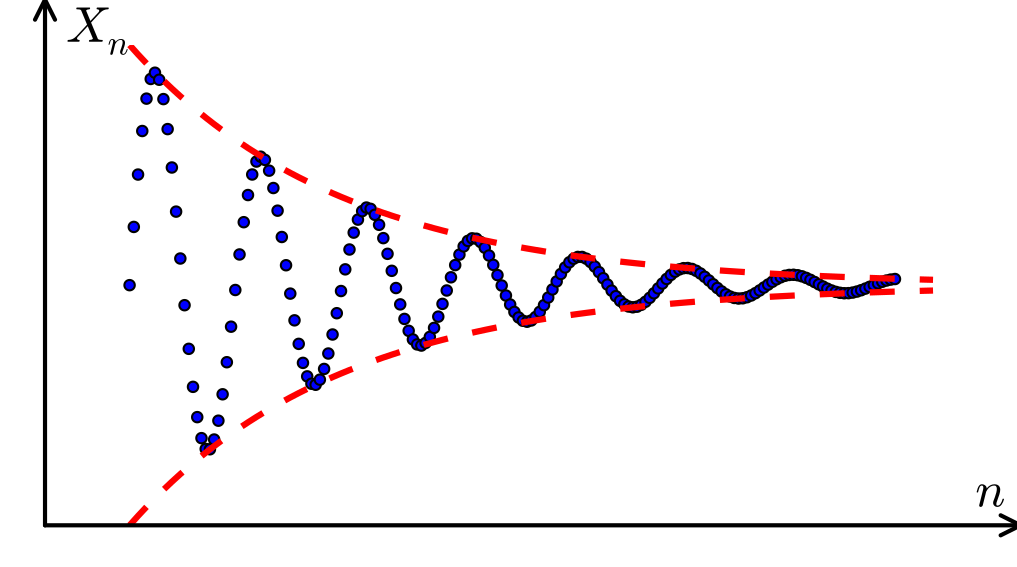
\includegraphics[width=6cm]{03-cauchy-1} }}%
	\hspace{5em}
	\subfloat[\centering Necauchyovská posloupnost]{{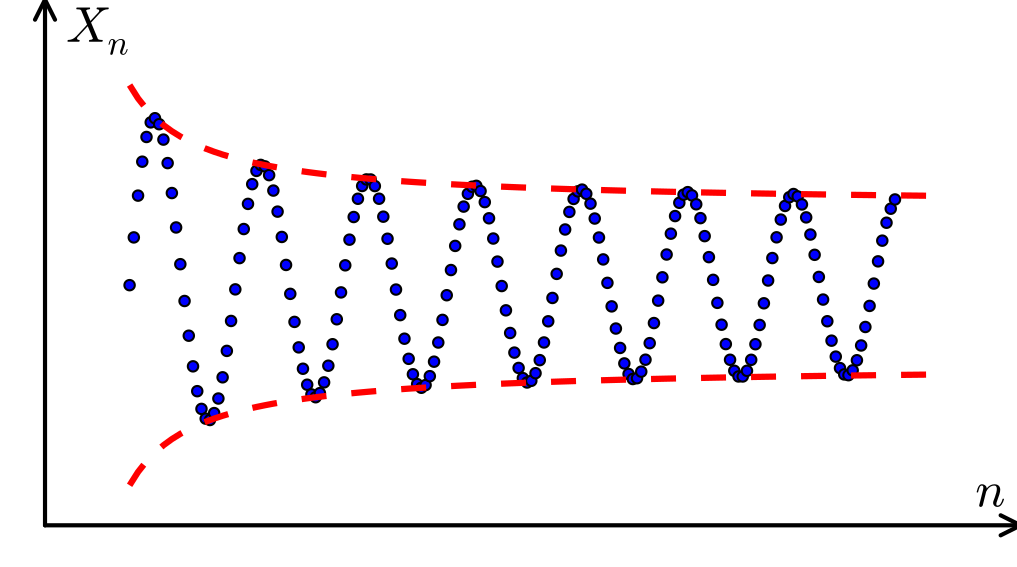
\includegraphics[width=6cm]{03-cauchy-2} }}%
	\caption{Příklady cauchyovské a necauchyovské posloupnosti}%
\end{figure}

\begin{lemma}[Konvergence cauchyovské posloupnosti]
	Nechť má cauchyovská posloupnost konvergentní podposloupnost. Potom posloupnost konverguje k limitě
	podposloupnosti.
\end{lemma}

\begin{proof}
	Nechť je $(x_n)_n$ cauchyovská posloupnost, $(x_{k_n})_n$ její podposloupnost a nechť $\lim_{n}(x_{k_n}) = x.$ Buď $d(x_m,x_n) < \varepsilon$ pro $ \forall m,n \geq n_1$ 
	a $d(x_{k_n},x) \leq \varepsilon$ pro $\forall n \geq n_2$. Položíme-li $n_0 = \max(n_1,n_2)$, máme pro $\forall n \geq n_0$ (protože $k_n \geq n$)
	\[d(x_n,x) \leq d(x_n,x_{k_n}) + d(x_{k_n},x) < 2\varepsilon.\]
	V první nerovnosti využíváme trojúhelníkovou nerovnost metriky.
\end{proof}

\begin{lemma}[Cauchyovská posloupnost součinu]
	Posloupnost $(x_{1}^{1}, ... , x_{n}^{1}), (x_{1}^{2},...,x_{n}^{2}), ...,(x_{1}^{k},...,x_{n}^{k}),...$
	je cauchyovská v $\prod_{i=1}^{n}(X_i, d_i)$ právě když každá z posloupností $(x_{i}^{k})_k$ je
	cauchyovská v $(X_i, d_i)$.
\end{lemma}

\begin{proof}
	\begin{itemize}
	    \item[ $\Rightarrow$:] Plyne bezprostředně z toho, že $d_i(u_i,v_i) \leq d((u_j)_j,(v_j)_j).$
	    \item[ $\Leftarrow$:] Nechť je každá $(x_i^k)_k$ cauchyovská. Pro $\varepsilon > 0$ a $i$ zvolme $k_i$ tak,
	    aby pro $k,l \geq k_i$ bylo $d_i(x_i^k, x_i^l) < \varepsilon.$ Potom pro $k,l \geq$ $\text{max}_i k_i$ máme 
	    \[d((x_1^k,...,x_n^k),(x_1^l,...,x_n^l)) < \varepsilon.\]
	\end{itemize}
\end{proof}

\subsection{Úplné metrické prostory}

\begin{definition}
	Metrický prostor $(X,d)$ je úplný, pokud v něm každá cauchyovská posloupnost konverguje.
\end{definition}

\begin{theorem}[Součin úplných prostorů]
	Součin úplných prostorů je úplný. Speciálně, $\mathbb{E}_n$ je úplný.
\end{theorem}

\begin{lemma}[Úplnost podprostoru]
	Podprostor úplného prostoru je úplný, právě když je uzavřený.
\end{lemma}

\begin{proof}
	\begin{enumerate}
		\item[$\Leftarrow \phantom{\lnot} $] Buď $Y \subseteq (X,d)$ uzavřený. Buď $(y_n)_n$ cauchyovská v $Y$. Potom je cauchyovská 
	    a tedy konvergentní v $X$ a kvůli uzavřenosti je limita v $Y$.
	    \item[$\lnot \Leftarrow \lnot $] Nechť $Y$ není uzavřený. Potom existuje posloupnost $(y_n)_n$ v $Y$ konvergentní v $X$ taková, že $\lim_n y_n \notin Y$.
	    Potom je $(y_n)_n$ cauchyovská v $X$ a jelikož je vzálenost stejná, též v $Y$. Ale v $Y$ nekonverguje.
	\end{enumerate}
\end{proof}

\begin{consequence}
	Podprostor $Y$ euklidovského prostoru $\mathbb{E}_n$ je úplný, právě když je uzavřený.
\end{consequence}

\begin{lemma}[Úplnost kompaktního prostoru]
	Každý kompaktní prostor je úplný.
\end{lemma}

\begin{proof}
	Cauchyovská posloupnost má podle kompaktnosti konvergentní podposloupnost a tedy konverguje.
\end{proof}

\end{document}
